\subsection{The Air Quality Index (AQI)}
The air quality index (AQI) is used to indicate the current air quality within a
standardized range. The AQI was established through the Clean Air Act in 1963.
The AQI is calculated from the amounts of particulate matter (PM$_{2.5}$ and
PM$_{10}$), ozone \ozone, carbon monoxide CO, sodium dioxide \sdo, and nitrogen
dioxide \ndo. The EPA sets standards for exposure levels for each of the gasses
based on scientific research. The levels can be advised over time. The range of
the index is from 0 to 500 with an AQI value of 100 being the national air
quality standard for each of the pollutants. Various levels have been defined
within 0 and 500 to indicate various health risks involved, as shown below:

\begin{figure}[h]
\centering
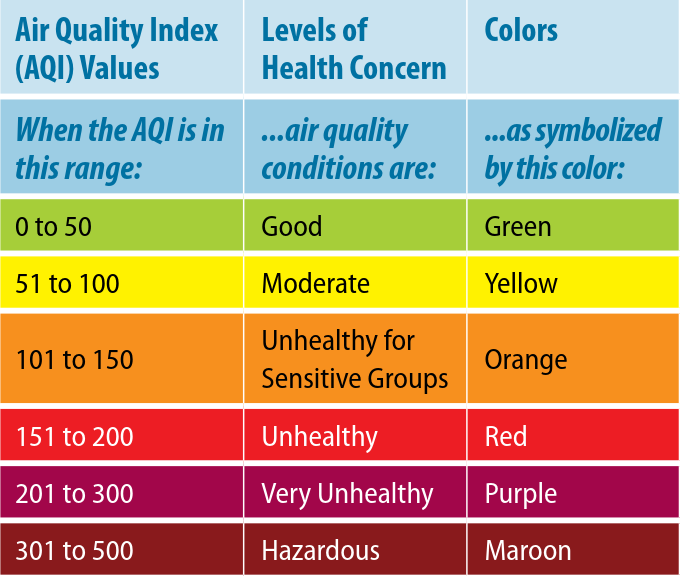
\includegraphics[scale=0.5]{aqi.png}
\caption{AQI Levels}
\label{fig:aqiLevels}
\end{figure}

